\section{Redes Sociais} \label{sec:socialnetworks}

As redes sociais\footnote{Neste contexto, o termo \emph{não} se refere a mídias sociais digitais como Facebook ou Instagram.} como tema de pesquisa vem recebendo crescente atenção nas décadas recentes. Seu principal potencial se encontra em sua capacidade de fomentar um aprofundamento maior no estudo das relações entre entidades e os padrões que tais conjuntos de relações produzem. Estes dois componentes formam o cerne da área de pesquisa de Análise de Redes Sociais; através dos mesmos, torna-se possível modelar e explorar fenômenos econômicos, sociológicos, logísticos e políticos, entre outros tópicos fundamentais no convívio humano e de outros seres sociais \cite{Wasserman1994}.

Segundo \citeonline{Wasserman1994}, estudos envolvendo a perspectiva de redes sociais apresentam características consideravelmente distintas de pesquisas habituais: enquanto estas geralmente preocupam-se com a medição e exploração de características individuais de uma amostra dos elementos de interesse (sejam estes pessoas, empresas, sindicatos, entre outros), a abordagem de redes sociais apresenta maior ênfase nos relacionamentos entre tais unidades, investigando características dos relacionamentos em si. Assim, pode-se dar atenção a aspectos como afinidade entre indivíduos, grau de concorrência entre empresas ou a influência que um líder possui sobre seus subordinados.

A Análise de Redes Sociais compreende um conjunto de conceitos primordiais cujas definições apresentam grande importância no desenvolvimento deste estudo e na análise dos trabalhos relacionados. Alguns dos principais conceitos, como especificado por \citeonline{Wasserman1994}, são:

\begin{alineas}
    \item Ator: representam as entidades individuais que se relacionam em uma rede social. Atores são frequentemente caracterizados como indivíduos, mas também podem representar empresas, departamentos, agências, entre outros;
    \item Laço: um relacionamento entre dois atores, o qual pode ser tanto imediato quanto longínquo. O significado de um laço apresenta grande variedade; exemplos incluem a afinidade entre indivíduos, a transferência de recursos materiais, afiliações, conexões entre locais físicos (como estradas ou pontes) e relações formais (como níveis hierárquicos em uma corporação). Laços podem ser tanto mútuos quanto unidirecionais.
    \item Díade: um par de atores, que podem ou não estar conectados por laços;
    \item Tríade: um conjunto de três atores e os possíveis laços entre eles;
    \item Subgrupo: um subconjunto dos atores de uma rede social e os laços formados entre eles. Essencialmente, uma generalização de díades e tríades, podendo conter um número arbitrário de atores;
    \item Grupo: grupos são caracterizados como conjuntos finitos de atores cujos laços passam por algum tipo de medição, apresentando algum nível de homogeneidade. Entretanto, a definição de grupo ainda é motivo de debate nos círculos de pesquisa sociológica devido à sua natureza abstrata;
    \item Relação: uma relação consiste na coleção de laços de um tipo específico entre os membros de um grupo; exemplos incluem os laços de parceria entre corporações ou as alianças estabelecidas entre países;
    \item Rede social: uma rede social é definida como um conjunto finito de grupos e as relações presentes sobre os tais. A maior parte dos estudos, assim como o presente, considera uma rede social \emph{unimodal}; ou seja, uma rede com apenas um grupo de atores, com uma ou mais relações.
\end{alineas}

A Figura \ref{fig:networkDefs} apresenta graficamente alguns dos termos definidos. Nesta, tem-se uma rede social com 34 atores, representados pelos círculos com preenchimento em azul petróleo, com seus laços -- todos mútuos -- sendo retratados por linhas retas cinzas. Em evidência, exibe-se uma díade (um par de atores) e uma tríade (um conjunto de três atores), sendo esta totalmente conectada.

\begin{figure}[ht]
    \centering
    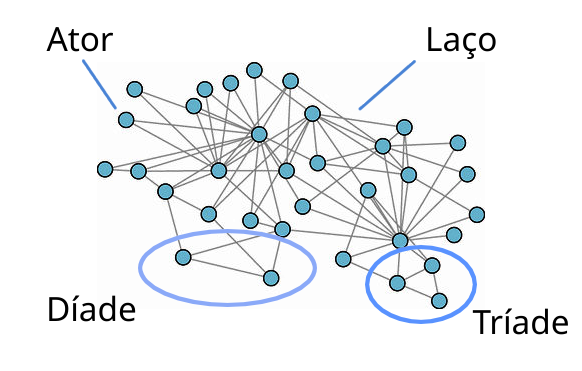
\includegraphics[width=8cm]{imagens/social_network.png}
    \caption{Representação de conceitos de redes sociais.}
    \label{fig:networkDefs}
    \Fonte{O autor.}
\end{figure}

Uma das características mais importantes de uma rede social é o padrão estrutural formado pela organização de seus laços. \citeonline{Christakis2007} indicam que o mesmo conjunto de indivíduos pode apresentar grande variabilidade no modo como completa uma tarefa de acordo com a forma com que seus laços estão organizados; desta maneira, uma rede social cuidadosamente estruturada pode ser tão eficaz quanto uma segunda rede com muito mais atores porém organizada aleatoriamente. Por exemplo, um exército organizado em pequenos esquadrões fortemente conectados apresenta uma efetividade muito superior a um arranjo em fila, onde cada soldado conhece apenas quem está atrás ou em sua frente.

A Figura \ref{fig:structures} apresenta três exemplos de organizações de redes sociais. A primeira, mais à esquerda, consiste em uma estrutura que se assemelha a uma longa fila com laços homogêneos, onde cada ator está ligado com exatamente outros dois atores, exceto pelo primeiro e pelo último; a segunda, no meio, apresenta uma estrutura hierárquica, onde um ator central possui laços dirigidos para outros dois atores, que por sua vez também estão ligados de forma dirigida com outros dois atores distintos, e assim sucessivamente; por fim, a terceira, à direita, apresenta uma rede social contendo dez subconjuntos de atores, cada um contendo dez atores completamente conectados por laços mútuos.

\begin{figure}[ht]
    \centering
    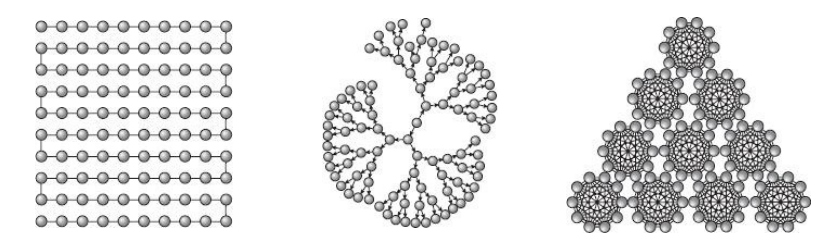
\includegraphics[width=15cm]{imagens/social_structures.png}
    \caption{Três exemplos de estruturas de redes sociais.}
    \label{fig:structures}
    \Fonte{\citeonline{Christakis2007}}
\end{figure}

Tais organizações manifestam-se com alguma frequência em situações sociais reais. Por exemplo, a estrutura hierárquica captura aspectos cruciais de estratégias de marketing multinível ou esquemas de pirâmide, onde há um ator central que detém controle sobre a disseminação de informações pela rede, enquanto a estrutura de subgrupos coesos pode representar uma estratégia de organização militar ou equipes de diferentes setores de uma empresa \cite{Christakis2007}.

Entretanto, no sentido geral, redes sociais tendem a evoluir de forma orgânica, e portanto não apresentam uma homogeneidade tão acentuada como nos exemplos citados. Alguns estudos buscaram investigar como esta evolução ocorre; um dos principais fenômenos identificados foi a \emph{homofilia}\footnote{tradução livre de \textit{homophily}}, que prescreve que indivíduos tendem a formar laços com outros que apresentam características similares \cite{McPherson2001}. Além disso, particularidades de cada indivíduo podem afetar de forma significativa a maneira como laços são formados: por exemplo, indivíduos de natureza introvertida podem tender a possuir círculos sociais menores, enquanto aqueles mais propícios a buscar novas experiências podem exibir uma quantidade de laços acima da média \textit{(ibidem)}.

A Figura \ref{fig:karate}, que exibe a rede de amizades em um clube de karatê de 34 membros, demonstra alguns destes aspectos: dois indivíduos, de identificadores 1 e 34, possuem um grande número de laços imediatos, enquanto outros -- como os atores 16, 15 e 23 -- possuem apenas dois laços imediatos.

\begin{figure}[ht]
    \centering
    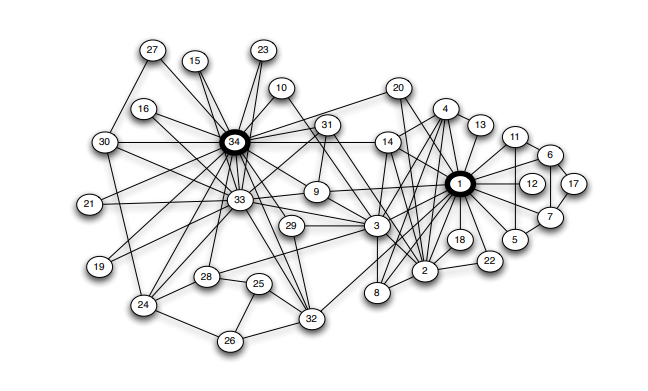
\includegraphics[width=15cm]{imagens/karate.png}
    \caption{Rede social de um clube de karatê}
    \label{fig:karate}
    \Fonte{\citeonline{Easley2010}}
\end{figure}

Apesar desta variabilidade, alguns estudos foram capazes de identificar alguns padrões na distribuição de laços em redes sociais. Um dos mais significativos foi o experimento conduzido por \citeonline{Milgram1967}, onde os participantes recebiam uma carta destinada a uma pessoa desconhecida e deveriam entregá-la a algum indivíduo próximo, que por sua vez deveria repassá-la da mesma forma até que a carta chegasse a seu destinatário. Analisando o percurso das cartas que não foram perdidas, o autor observou que a maioria delas necessitou de aproximadamente seis repasses, descrevendo assim o Fenômeno do Mundo Pequeno e cunhando a expressão "seis graus de separação".

Ao longo do restante desta seção, dará-se maior ênfase na descrição dos processos de disseminação de influência através de redes sociais, assim como algumas características de grupos sociais no contexto educacional.

\subsection{Influência Social e seus Efeitos} \label{sec:socialinfluence}

Segundo \citeonline{Simons-Morton2010}, a influência social representa o efeito que outros causam sobre os comportamentos e atitudes de indivíduos ou grupos. A influência pode originar-se tanto de pessoas muito próximas, com as quais o invidíduo em questão possui um relacionamento íntimo, quanto de pessoas mais distantes, com as quais existe um laço social direto porém o mesmo não é muito intenso \cite{Berkman2000}. Entretanto, até mesmo pessoas desconhecidas podem causar algum nível de influência; uma demonstração deste fenômeno foi relatada na pesquisa de \citeonline{Fowler2008}, que identificou que a disseminação de felicidade em uma rede estudada durante 20 anos se estende por até três graus de separação (ou seja, pode advir de amigos de amigos de amigos). Na figura \ref{fig:socialzones}, tem-se uma representação das zonas de contato social entre indivíduos.

\begin{figure}[ht]
    \centering
    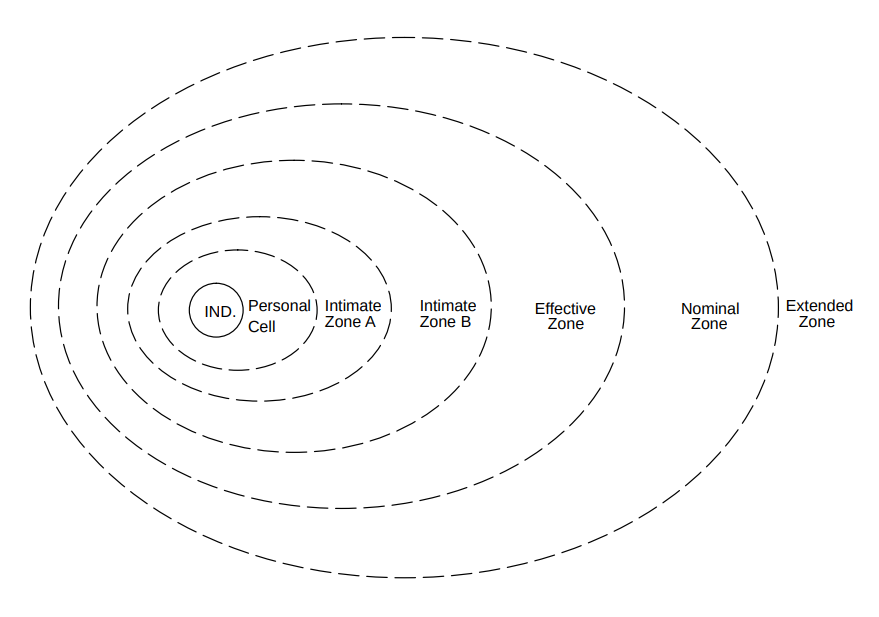
\includegraphics[width=12cm]{imagens/zones.png}
    \caption{Zonas de contato social.}
    \label{fig:socialzones}
    \Fonte{\citeonline{Berkman2000}}
\end{figure}

O modelo apresentado pela figura foi descrito por \citeonline{Berkman2000} com base em outros estudos sobre influência social e níveis de contato. Neste modelo, tem-se seis zonas sociais: (i) \textit{personal cell} (célula pessoal), que representa os familiares mais próximos e os mais íntimos dos amigos; (ii) \textit{intimate zone A} (zona íntima A), que representa familiares próximos e amizades íntimas ativas; (iii) \textit{intimate zone B} (zona íntima B), que consiste em familiares e amigos emocionalmente importantes mas com um cunho mais passivo; (iv) \textit{effective zone} (zona efetiva), composta por pessoas com as quais o relacionamento é mantido devido a razões de necessidade cotidiana; (v) \textit{nominal zone} (zona nominal), que contém apenas pessoas que o indivíduo conhece mas que não apresentam grande importância; e (vi) \textit{extended zone} (zona estendida), que consiste em pessoas distantes com as quais não há quase nenhum contato, porém o indivíduo em questão as conhece pelo menos de rosto.

\citeonline{Berkman2000} argumenta que todas as zonas do modelo apresentam importância considerável, não somente os círculos mais internos. Apesar de estes serem extremamente importantes para a manutenção da saúde emocional, indivíduos que pertencem à zona efetiva, nominal ou estendida fornecem suporte instrumental -- ou seja, auxiliam na execução de alguma tarefa ou na conquista de algum objetivo. Assim, tais indivíduos podem causar mudanças de comportamento e portanto também são agentes de influência social, mesmo que de forma menos acentuada.

Tratando das consequências da influência social, \citeonline{Steinberg2007} relatam que, assim como outros estudos conduzidos previamente evidenciaram, a adoção de hábitos perigosos e nocivos -- como abuso de substâncias, delinquência e imprudência no trânsito -- aumenta significativamente no período da adolescência, primariamente devido à maior susceptibilidade a pressão de pares, e estabiliza à medida que o indivíduo atinge a idade adulta.

Entretanto, este padrão também se mantém para condutas neutras ou até mesmo socialmente valorizadas, como tirar notas boas ou evitar drogas. Os autores sugerem que tal comportamento pode ser causado pela noção de que os pares de um indivíduo representam um ponto de referência comportamental que deve ser seguido, caracterizando o grupo social como um ambiente que tende à homogeneidade -- em caso de visões conflitantes, o indivíduo que foge à regra pode sofrer uma série de efeitos negativos, como rejeição, ostracismo e exclusão do grupo \cite{Steinberg2007,Gremmen2017}.

\subsection{Redes Sociais no Contexto Educacional} \label{sec:networkseducation}

A influência social e a disseminação de comportamento também causam profundos efeitos sobre os hábitos de estudantes, especialmente devido à grande quantidade de tempo que estes passam interagindo com seus colegas de classe, sendo esta uma característica observada principalmente no período da adolescência \cite{Butler-Barnes2015}. Na literatura científica, tem-se um considerável arcabouço de estudos que investigam padrões de características de propagação de influência e de que forma seus efeitos se manifestam nos estudantes, buscando correlações entre seu contexto social e outras variáveis de interesse \cite{Flashman2012,Gremmen2017,Farmer1996,Blansky2013,Rambaran2017,Berndt1990}.

\citeonline{Goodenow1993} argumentam que a motivação acadêmica não pode ser analisada como um fenômeno exclusivamente individual, pois este é afetado profundamente pelas relações sociais e laços de amizade dos estudantes. As autoras também sugerem que a sensação de pertencimento à escola e a influência dos valores de amigos são fatores altamente importantes quando se trata de motivação acadêmica, sendo que este último apresenta um nível de correlação levemente inferior -- porém, no quesito da valorização das atividades acadêmicas, a influência das amizades apresentou correlação elevada. O estudo também identificou que o impacto do pertencimento é mais significativo em grupos com maior risco de evasão escolar.

Reforçando a noção do impacto do contexto social de estudantes sobre seu comportamento escolar, \citeonline{Rice2013} identificaram que alunos relatam atitudes e percepções mais positivas, além de maior autoconfiança, acerca do estudo de matemática e ciências quando estes recebem suporte social abundante de seus seus pais, professores e amigos. O trabalho identificou que todos os três fatores apresentam correlações similares entre si (sendo todas positivas e estatisticamente significantes), porém o relato dos alunos amostrados sugere que o suporte social do grupo de amigos é consideravelmente inferior ao suporte oferecido por pais e professores. Sendo assim, sugere-se que a influência de laços de amizade merece um estudo mais aprofundado, por ser um fator destoante dos demais.